\chapter{Path Indexing}
In this section we give an informal overview of path indexing and take a closer look at some details of its implementation in Isabelle/ML.\\
A path index is used to store a collection of terms for efficient querying. The queries commonly include retrieval of generalisations or unifiables of a term from the collection.\\
The core concept on which path indexing is based is the mapping of each symbol in a term to a path. This path consists of the nodes traversed from the root to the symbol. In the standard tree form this is an alternating sequence of symbols and the index of the argument which is traversed next. Additionally this path starts with the root symbol and ends with the symbol being addressed. As a result a single term is described by a collection of paths.\\
\begin{figure}[h]
\centering
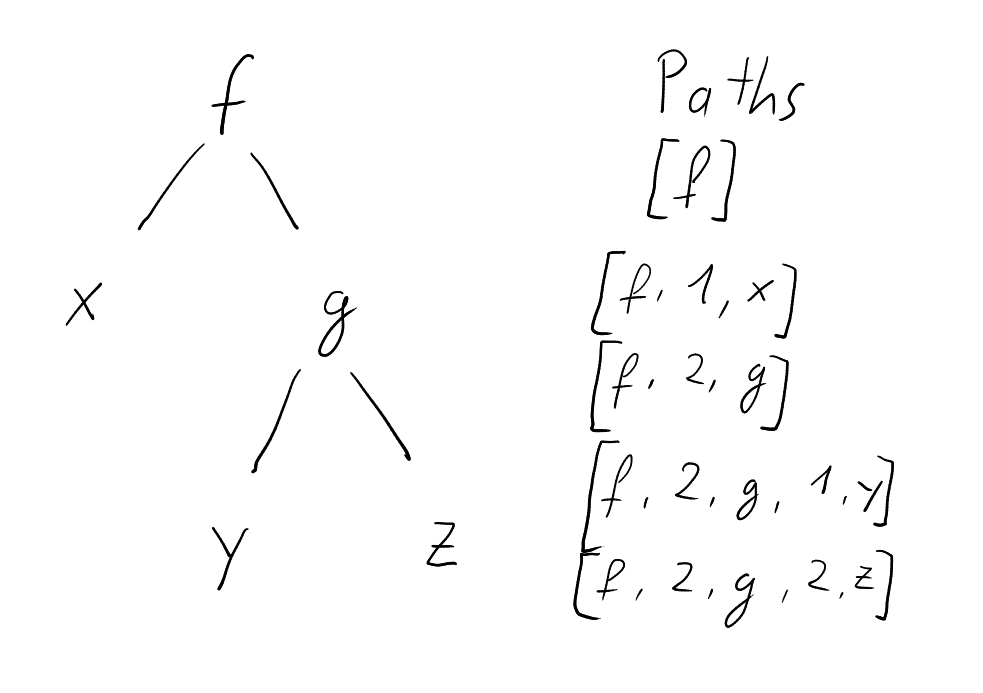
\includegraphics[scale=0.25]{figures/term_path.png}
\caption{A term and the paths associated with its symbols}
\end{figure}\\
To store the paths of different terms within one index we must associate each path with a list of terms within which this path occurs. These are called path lists. As a term is described by a path for each symbol each term is generally saved in many path lists.\\
The queries are based on intersections and unions of the different path lists to enforce constraints on the terms. The simplest query is the lookup of identical terms, for example to check if a term is already contained within the index. To answer the query we first build a list of the paths the term contains. Next we lookup the path lists corresponding to them in the index. The intersection of these path lists returns all terms containing symbols at identical paths as the query term. Under the assumption of type correctness/soundness \todo{Test}
A query for variants of a term is resolved by collecting the path lists associated with each symbol. These path lists are then intersected to retain only those terms that have identical symbols at all positions. More complex queries like instances, generalisations and unifiables are handled by introducing unions of two recursive calls or ignoring variables.\\
The queries are not exact and may return extra terms. For example an index containing both ``f x'' and ``f x y'' will return both terms when queries for variants of ``f x''. This is consequence of the fact that the total number of arguments of a function is not stored and ``f x y'' matches ``f x'' on all its symbols. Additionally the name of variables is not stored as all queries except the lookup handle them indifferently which reduces the number of unions required.\\
